\documentclass[a4paper, twocolumn]{article}

%\setlength{\parskip}{0.5\baselineskip}
\usepackage{pdfpages}

\usepackage{geometry}
% \geometry{left = 2.54 cm, right = 2.54 cm, top = 2.54 cm, bottom = 2.54 cm}
\geometry{left = 1 cm, right = 1 cm, top = 1 cm, bottom = 1 cm}

\usepackage{setspace}
\renewcommand{\baselinestretch}{1.0}
\usepackage{indentfirst}
\setlength{\parindent}{2em}

%\usepackage{fontspec}
%\setmainfont{Times New Roman}

\usepackage{ulem}
\usepackage{graphicx}
%\usepackage{wrapfig}
\usepackage{enumerate}
\usepackage{xcolor}
%\usepackage{subcaption}
\usepackage{float}
\usepackage{amsmath, amssymb, amsthm}
\usepackage{booktabs}

\pagestyle{empty} % Not showing page number

\begin{document}
\renewcommand{\thesection}{\Roman{section}}
\renewcommand{\thesubsection}{\Alph{subsection}}
\renewcommand{\thesubsubsection}{\thesubsection.\arabic{subsubsection}}
\renewcommand{\d}{\: \mathrm{d} }
\newcommand{\e}{\mathrm{e}}

\section{Chapter 6}
    Excess minority carrier lifetime:
    \begin{equation*}
        \begin{aligned}
            \frac{\d (\delta n(t))}{\d t} &= - \alpha_r (p_0 + n_0) \delta n(t) \\
            \tau &= \frac{1}{\alpha_r (n_0 + p_0)}
        \end{aligned}
    \end{equation*}
    \par n-type:
    \begin{equation*}
        R^\prime_n = R^\prime_p = \frac{\delta p(t)}{\tau_{p0}}
    \end{equation*}
    \par p-type:
    \begin{equation*}
        R^\prime_n = R^\prime_p = \frac{\delta n(t)}{\tau_{n0}} 
    \end{equation*}
    
    \par Quasi-Fermi Energy Level
    \begin{equation*}
        \begin{aligned}
            n_0 + \delta n &= n_i \exp \left( \frac{E_{Fn} - E_{Fi}}{kT}  \right) \\
            p_0 + \delta p &= n_i \exp \left( \frac{E_{Fi} - E_{Fp}}{kT}  \right) \\
        \end{aligned}
    \end{equation*}
    % \begin{figure}[H]
    % \begin{minipage}{\linewidth}
        % \centering
        \includegraphics[width=0.8\linewidth]{Quasi-fermi-level-1.jpg}\\
    % \end{minipage}
        % \label{fig:Quasi-fermi-level.jpg}
    % \end{figure}
    
    \par Excess Carrier Lifetime
    % \begin{enumerate}
    %     \item Capture of an electron form conductance band by an initially neutral empty trap
    %     \begin{equation*}
            
    %     \end{equation*}
    % \end{enumerate}
    % \begin{equation*}
    %     \boxed{R_n = R_p = \frac{C_n C_p N_t (np - n_i^2)}{C_n (n + n^\prime) + C_p(p + p^\prime)} \equiv R}
    % \end{equation*}
    % where 
    % \begin{equation*}
    %     \resizebox*{0.8\linewidth}{!}{ %
    %          n^\prime &= N_c \exp\left[ - \dfrac{E_c - E_t}{kT}  \right], \quad  p^\prime &= N_v \exp \left[ - \dfrac{E_t - E_v}{kT}  \right]   
    %      }
    % \end{equation*}
    \begin{equation*}
        % \boxed{
            \begin{aligned}
                R_n = R_p &= \frac{C_n C_p N_t (np - n_i^2)}{C_n (n + n^\prime) + C_p(p + p^\prime)} \\
                &= \frac{(np - n_i^2)}{\tau_{p0}(n + n^\prime) + \tau_{n0} (p + p^\prime) } 
            \end{aligned}
            % }
    \end{equation*}
    where \\
    % \begin{equation*}
        \resizebox*{\linewidth}{!}{ %
            $n^\prime = N_c \exp\left[ - \dfrac{E_c - E_t}{kT}  \right], p^\prime = N_v \exp \left[ - \dfrac{E_t - E_v}{kT}  \right], \text{ and } \tau_{n0} = \dfrac{1}{C_n N_t}$
        }
    % \end{equation*}
    
    \par Surface Effects
    \begin{equation*}
        \begin{aligned}
            - D_p \left. \left[ \hat{n} \cdot \frac{\d (\delta p)}{\d x}  \right] \right|_{\text{surf}} = s \; \delta p |_{\text{surf}}
        \end{aligned}
    \end{equation*}
    \begin{equation*}
        \begin{aligned}
            \delta p(x) = g^\prime \tau_{p0} \left( 1 - \frac{sL_p\e^{-x/L_p} }{D_p + sL_p}  \right)
        \end{aligned}
    \end{equation*}
    
    \par Time-dependent Continuity Equation
    \begin{equation*}
        \begin{aligned}
            \frac{\d p}{\d t} = - \frac{F_p^+}{\d x} + g_p - \frac{p}{\tau_{pt}}
        \end{aligned}
    \end{equation*}
    \begin{equation*}
        % \boxed{
            \begin{aligned}
                D_n \frac{\d^2 n}{\d x^2} + \mu_n \left( E \frac{\d n}{\d x} + n \frac{\d E}{\d x}  \right) + g_n - \frac{n}{\tau_{nt}} = \frac{\d n}{\d t} \\
                D_p \frac{\d^2 p}{\d x^2} - \mu_p \left( E \frac{\d p}{\d x} + p \frac{\d E}{\d x}  \right) + g_p - \frac{p}{\tau_{pt}} = \frac{\d p}{\d t} \\
            \end{aligned}
        % }
    \end{equation*}
    % \par For homogeneous semiconductor, $n(x) = n_0 + \delta n(x)$, the equation can be simplified to 
    \begin{equation*}
        % \boxed{
            \begin{aligned}
                D_n \frac{\d^2 (\delta n)}{\d x^2} + \mu_n \left( E \frac{\d (\delta n)}{\d x} + n \frac{\d E}{\d x}  \right) + g_n - \frac{n}{\tau_{nt}} &= \frac{\d (\delta n)}{\d t} \\
                D_p \frac{\d^2 (\delta p)}{\d x^2} - \mu_p \left( E \frac{\d (\delta p)}{\d x} + p \frac{\d E}{\d x}  \right) + g_p - \frac{p}{\tau_{pt}} &= \frac{\d (\delta p)}{\d t} \\
                g_n - \frac{n}{\tau_{nt}} &= g^\prime - \frac{\delta n}{\tau_{nt}}
            \end{aligned}
        % }
    \end{equation*}
    
    % \begin{figure}[H]
    %     \centering
        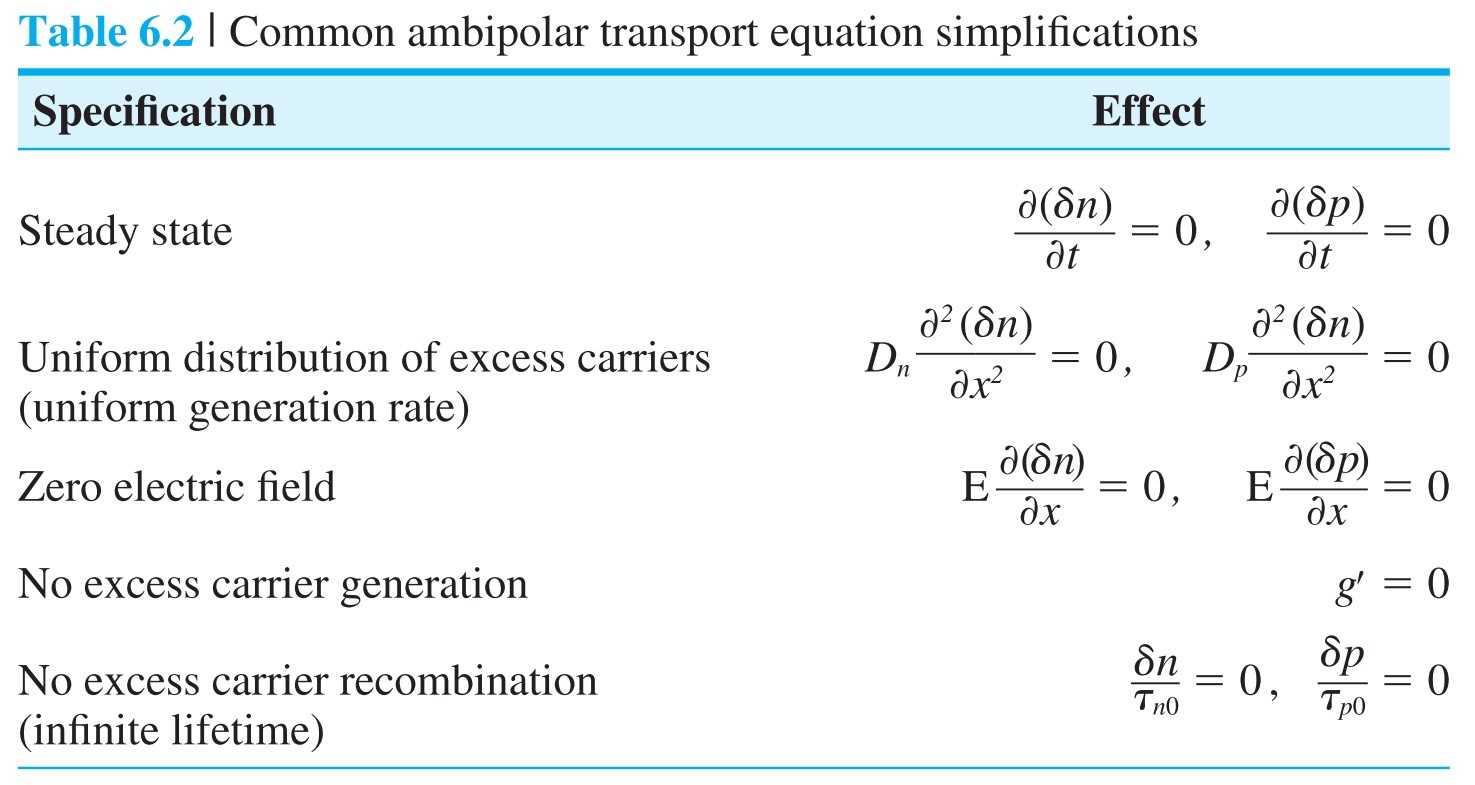
\includegraphics[width=0.9\linewidth]{Equation-simplification.jpg}
    %     \label{fig:Equation-simplification.jpg}
    % \end{figure}
    
    % \newpage
    \par General solutions:
    \begin{itemize}
        \item 
            \begin{equation*}
                \frac{\d (\delta p)}{\d t}  = - \frac{\delta p}{\tau_{p0}} 
            \end{equation*}
            solution:
            \begin{equation*}
                \color{magenta} \delta p(t) = \delta p(0) \e^{- t/ \tau_{p0}} 
            \end{equation*}
        \item 
            \begin{equation*}
                g^\prime - \frac{\delta p}{\tau_{p0}} = \frac{\d (\delta p)}{\d t}  
            \end{equation*}
            solution:
            \begin{equation*}
                \color{magenta} \delta p(t) = g^\prime \tau_{p0} \left( 1 - \e^{- t / \tau_{p0}}  \right)
            \end{equation*}
        \item 
            \begin{equation*}
                D_n \frac{\d ^2 (\delta n)}{\d x^2} - \frac{\delta n}{\tau_{n0}} = 0
            \end{equation*}
            solution:
            \begin{equation*}
                \color{magenta}
                \delta n(x) = A \e^{- x/L_n} + B \e^{x/L_n}, \quad L_n = \sqrt{D_n \tau_{n0}}
            \end{equation*}
            special:
            \begin{equation*}
                \color{magenta}
                \delta n(x) = 
                \left\{
                    \begin{aligned}
                        \delta n(0) \e^{-x / L_n}, &x \ge 0 \\
                        \delta n(0) \e^{+x/L_n}, &x \le 0
                    \end{aligned}
                \right.
            \end{equation*}
        \item 
            \begin{equation*}
                D_p \frac{\d ^2 \delta p}{\d x^2} - \frac{\delta p}{\tau} + G_{ex} = 0
            \end{equation*}
            solution:
            \begin{equation*}
                \color{magenta}
                \delta p(x) = A \exp(\lambda x) + g \tau, \quad \lambda = \pm \frac{1}{\sqrt{D_p \tau}} 
            \end{equation*}
        \item 
            \begin{equation*}
                D_p \frac{\d^2 (\delta p)}{\d x^2} - \mu_p E_0 \frac{\d (\delta p)}{\d x} - \frac{\delta p}{\tau_{p0}} = \frac{\d (\delta p)}{\d t}  
            \end{equation*}
            solution:
            \begin{equation*}
                \color{magenta}
                \delta p(x, t) = \frac{\e^{-t/\tau_{p0}} }{\left( 4 \pi D_p t \right)^{1/2}} \exp\left[ \frac{-\left(x - \mu_p E_0 t\right)^2}{4 D_p t}  \right]
            \end{equation*}
        \item 
            \begin{equation*}
                D_p \frac{\d^2 \delta p}{\d x^2} - \mu_p E \frac{\d \delta p}{\d x} - \frac{\delta p}{\tau} = 0 
            \end{equation*}
            solution: \\
            \begin{minipage}{\linewidth}
                \resizebox*{\textwidth}{!}{
                    $
                        \color{magenta}
                        \begin{aligned}
                            & \delta p(x) = A \exp\left( \lambda x \right) + C \\
                            & \lambda = \frac{L_p(E) \pm \sqrt{L_p^2 (E) + 4 L_p^2}}{2 L_p^2},\quad L_p = \sqrt{\tau D_p},\quad L_p(E) = \tau \mu_p E
                        \end{aligned}
                    $
                }
            \end{minipage}
            special:\\
            \begin{minipage}{\linewidth}
                \resizebox*{\textwidth}{!}{ %
                    $
                    \color{magenta}
                    \delta p(x) = \delta p(0) \exp \left[ \dfrac{L_p(E) \pm \sqrt{L_p^2 (E) + 4 L_p^2}}{2 L_p^2} x \right] = \left\{
                        \begin{aligned}
                            &\delta p(0) \exp \left( - \dfrac{x}{L_p}  \right), &\text{ if } L_p(E) \ll L_p \\
                            &\delta p(0) \exp \left( - \dfrac{x}{L_p(E)}  \right), &\text{ if } L_p(E) \gg L_p
                        \end{aligned}
                    \right.
                    $
                }
            \end{minipage}
    \end{itemize}
    
% \newpage
\section{Chapter 7}
    % \begin{figure}[H]
        % \centering
        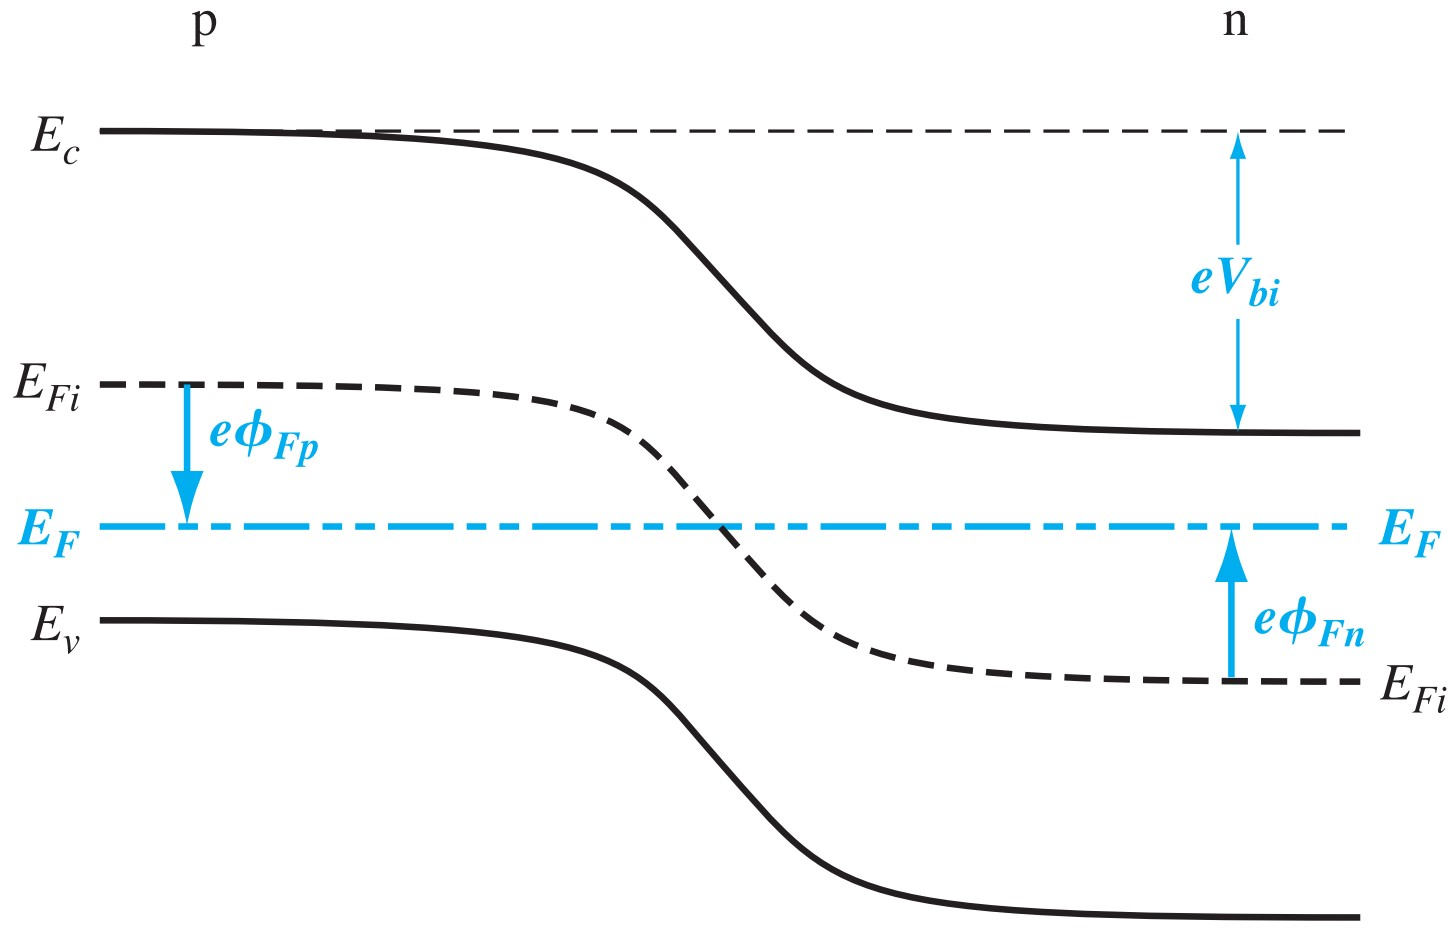
\includegraphics[width=0.6\linewidth]{pn-junction-energy-band-diagram.jpg} \\
    % \end{figure}
    $V_{bi}$: built-in potential barrier.
    \begin{equation*}
        \begin{aligned}
            V_{bi} &= |\phi_{Fn}| + |\phi_{Fp}| \\
            &= \frac{kT}{e} \ln \left( \frac{N_a N_d}{n_i^2}  \right) = V_t \ln\left( \frac{N_a N_d}{n_i^2}  \right)
        \end{aligned}
    \end{equation*}
    $V_t = kT / e$ defined as the thermal voltage.

    \begin{minipage}{\linewidth}
        \hspace{-1cm}
        \begin{minipage}[b]{0.49\linewidth}
            % \begin{figure}[H]
                % \centering
                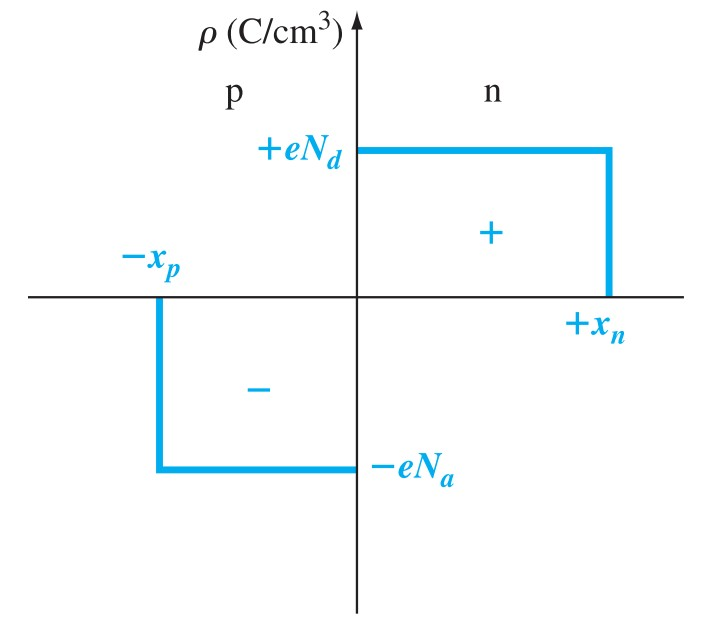
\includegraphics[width=0.95\linewidth]{Space-charge-density.jpg} \\
            % \end{figure}
            \begin{equation*}
                N_a x_p = N_d x_n
            \end{equation*}
        \end{minipage}
        \begin{minipage}[b]{0.49\linewidth}
            % \begin{figure}[H]
                % \centering
                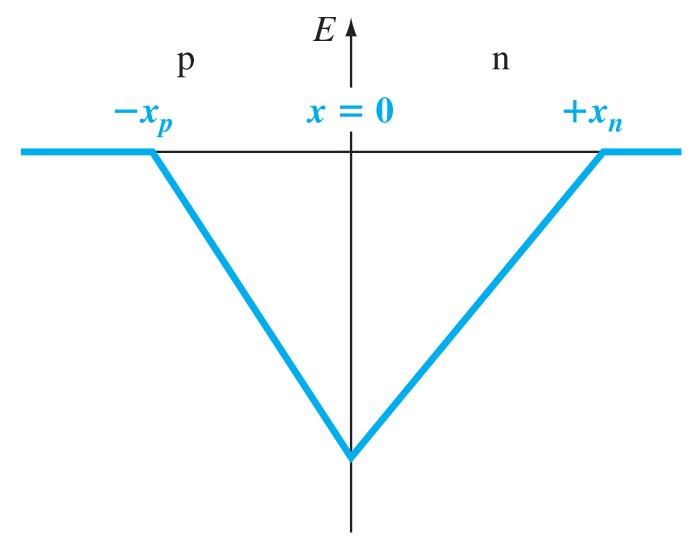
\includegraphics[width=0.95\linewidth]{pn-junction-electric-field.jpg}\\
            % \end{figure}
            \begin{equation*}
                |k| = \frac{e N_{a/d}}{\varepsilon_s} 
            \end{equation*}
        \end{minipage}
    \end{minipage}
    
        % \resizebox{\linewidth}{!}{
    % \fbox{
        % \begin{minipage}{0.95\linewidth}
        % \hspace{-1cm}
            \begin{equation*}
                N_a x_p = N_d x_n
            \end{equation*}
            \begin{equation*}
                \begin{aligned}
                    x_n &= \sqrt{\frac{2 \varepsilon_s \left( V_{bi} + V_R \right)}{e} \left[ \frac{N_a}{N_d}  \right]\left[ \frac{1}{N_a + N_d}  \right]} \\
                    x_p &= \sqrt{\frac{2 \varepsilon_s \left( V_{bi} + V_R \right)}{e} \left[ \frac{N_d}{N_a}  \right]\left[ \frac{1}{N_a + N_d}  \right]}
                \end{aligned}
            \end{equation*}
            \par $\varepsilon_s = \varepsilon_r \varepsilon_0$, where $\varepsilon_0 = 8.85 \times 10^{-14} F \cdot cm^{-1}$.
            \par $\varepsilon_r = 11.7$ for $Si$.
    
            \begin{equation*}
                W = x_n + x_p = \sqrt{\frac{2 \varepsilon_s \left( V_{bi} + V_R \right)}{e}  \left[ \frac{N_a + N_d}{N_a N_d}  \right]}
            \end{equation*}
        % \end{minipage}
    % }
        % }
    % \fbox{
        % \resizebox{\linewidth}{!}{
        % \begin{minipage}{0.95\linewidth}
            \begin{equation*}
                E = \left\{
                    \begin{aligned}
                        - \frac{eN_a}{\varepsilon_s} (x + x_p),\quad & - x_p \le x \le 0 \\
                        - \frac{eN_d}{\varepsilon_s} (x_n - x),\quad & 0 \le x \le x_n  
                    \end{aligned}
                \right.
            \end{equation*}
            \begin{equation*}
                \begin{aligned}
                    |E_{max}| &= - \frac{eN_d x_n}{\varepsilon_s} = - \frac{e N_a x_p}{\varepsilon_s} \\ 
                    &= - \frac{2 (V_{bi} + V_R)}{W} 
                \end{aligned}
            \end{equation*}
            \begin{equation*}
                \phi(x) = - \int E(x) \d x
            \end{equation*}
        % \end{minipage}
        % }
    % }
    \par Junction Capacitance
    \begin{equation*}
        C^\prime = \frac{\d Q^\prime}{\d V} = \sqrt{\frac{e \varepsilon_s N_a N_d}{2 (V_{bi} + V_R) (N_a + N_d)} } = \frac{\varepsilon_s}{W}
    \end{equation*}
    
    \par One-sided Junction - p$^+$n junction:
    \begin{equation*}
        \begin{aligned}
            & x_{p} \ll x_n \\
            & W \approx x_n \\
            & C^\prime \approx \sqrt{\frac{e \varepsilon_s N_d}{2 (V_{bi} + V_R)} } \\
            & \left( \frac{1}{C^\prime}  \right)^2 = \frac{2(V_{bi} + V_R)}{e \varepsilon_s N_d} 
        \end{aligned}
    \end{equation*}
    % \begin{figure}[H]
    %     \centering
    \begin{center}
        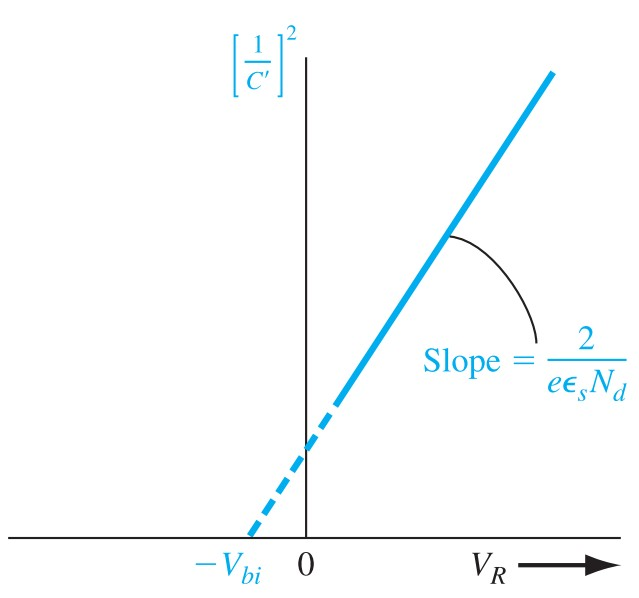
\includegraphics[width=0.4\linewidth]{C-versus-VR.jpg} \\
    \end{center}
        % \caption{$(1/C^\prime)^2$ versus $V_R$ of a uniformly doped pn junction}
        % \label{fig:C-versus-VR.jpg}
    % \end{figure}
    
\section{Chapter 8}
    % \begin{figure}[H]
    %     \centering
        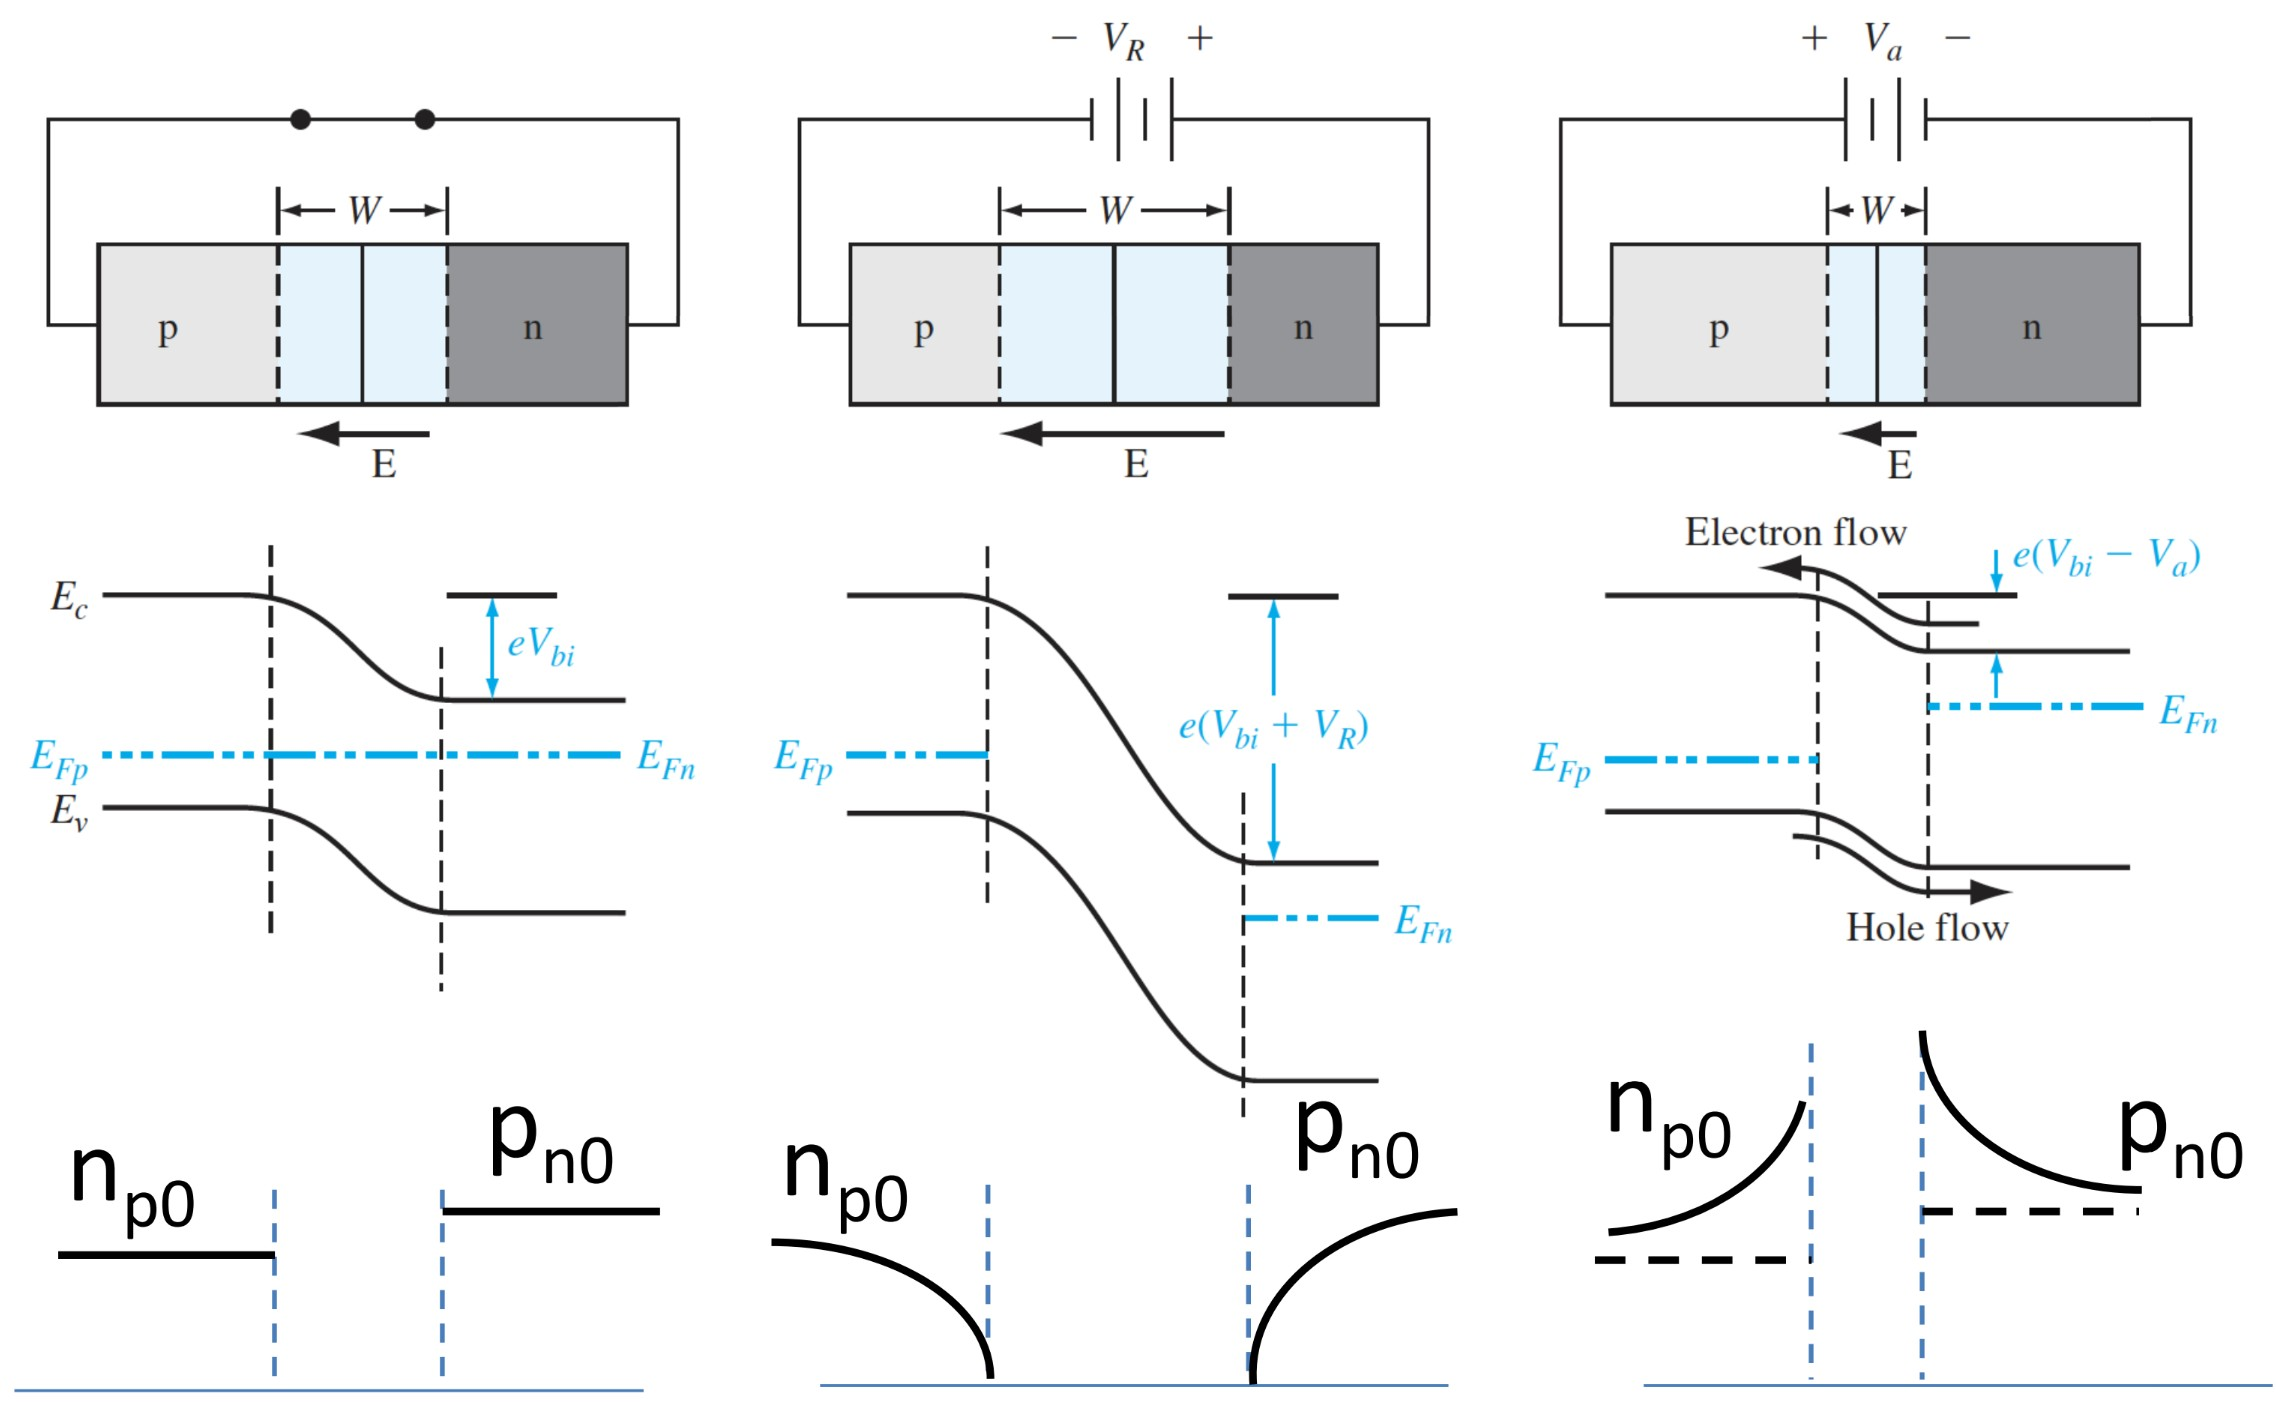
\includegraphics[width=0.8\linewidth]{Charge-flow-in-pn-junction.jpg} \\
    %     \label{fig:Charge-flow-in-pn-junction.jpg}
    % \end{figure}
    \begin{equation*}
        \begin{aligned}
            n_{p0} &= n_{n0} \exp\left( -\frac{e V_{bi} }{kT}  \right) \\
            p_{n0} &= p_{p0} \exp\left( -\frac{e V_{bi} }{kT}  \right) \\
        \end{aligned}
    \end{equation*}
    \par Forward biased
    \begin{equation*}
        \begin{aligned}
            n_{p} &= n_{p0} \exp\left( \frac{e V_{a} }{kT}  \right) \\
            p_{n} &= p_{n0} \exp\left( \frac{e V_{a} }{kT}  \right) \\
        \end{aligned}
    \end{equation*}
    \begin{equation*}
        \begin{aligned}
            \delta p_n(x) &= p_n(x) - p_{n0}  \\ &= p_{n0} \left[ \exp\left( \dfrac{eV_a}{kT} \right) - 1\right] \exp\left( \dfrac{x_n - x}{L_p}  \right), \quad x \ge x_n \\
            \delta n_p(x) &= n_p(x) - n_{p0}  \\ &= n_{p0} \left[ \exp\left( \dfrac{eV_a}{kT}  \right) - 1 \right] \exp \left( \dfrac{x_p + x}{L_n}  \right), \quad x \le - x_p \\
        \end{aligned}
    \end{equation*}
    % \begin{figure}[H]
    %     \centering
        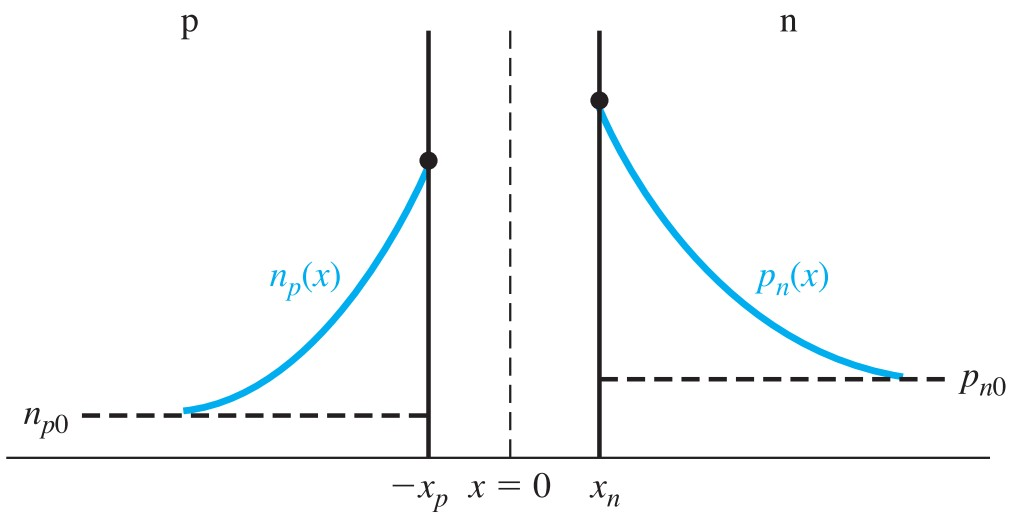
\includegraphics[width=0.6\linewidth]{Forward-biased-solution.jpg} \\
    %     \label{fig:Forward-biased-solution.jpg}
    % \end{figure}
    \par Quasi-Fermi Level \\
    % \begin{figure}[H]
    %     \centering
        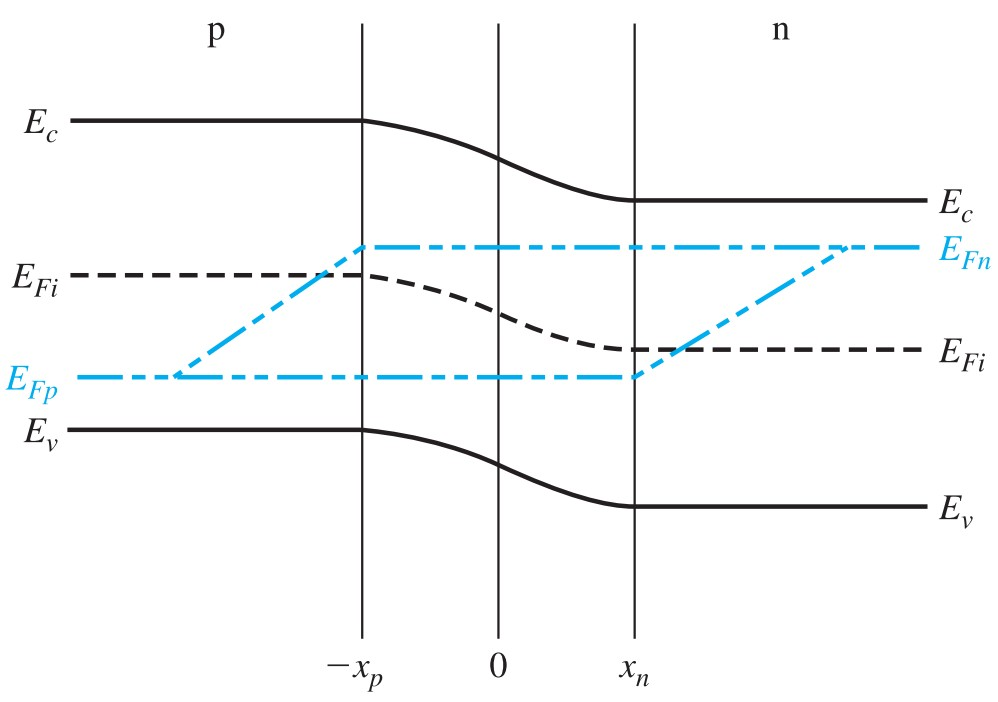
\includegraphics[width=0.6\linewidth]{Quasi-fermi-level.jpg}\\
    % \end{figure} 
    \begin{equation*}
        p = p_0 + \delta p = n_i \exp\left( \frac{E_{Fi} - E_{Fp} }{kT}  \right)
    \end{equation*}
    \begin{equation*}
        np = n_i^2 \exp \left( \frac{E_{Fn} - E_{Fp} }{kT}  \right)
    \end{equation*}
    \par Durrent density
    \begin{equation*}
        \begin{aligned}
            J_n(x) &= \frac{e D_n n_{p0}}{L_n} \left[ \exp \left( \frac{e V_a}{kT} \right) - 1 \right] \exp \left( \frac{x_p + x}{L_n} \right) \\
            J_p(x) &= \frac{e D_p p_{n0}}{L_p} \left[ \exp \left( \frac{e V_a}{kT} \right) - 1 \right] \exp \left( \frac{x_n - x}{L_p} \right) \\
        \end{aligned}
    \end{equation*}
    
    \par Ideal pn junciton current
    \begin{equation*}
        \begin{aligned}
            J &= J_s \left[ \exp\left( \frac{eV_a}{kT}  \right) - 1 \right] \\
            & \qquad  \text{where } J_s = \left[ \frac{eD_p p_{n0} }{L_p} + \frac{eD_n n_{p0} }{L_n}  \right] \\
            & \qquad \qquad \qquad   =en_{i}^{2}\left[\frac{1}{N_{a}} \sqrt{\frac{D_{n}}{\tau_{n 0}}}+\frac{1}{N_{d}} \sqrt{\frac{D_{p}}{\tau_{p 0}}}\right]
        \end{aligned}
    \end{equation*}
    
    \par Non-ideal I - Generation-recombination currents
    \begin{equation*}
        \begin{aligned}
            R_n &= \frac{(np - n_i^2)}{\tau_p \left[ n + n_i \exp \left( \frac{E_t - E_i}{kT}  \right) \right] + \tau_n \left[ p + n_i \exp \left( \frac{E_i - E_t}{kT}  \right) \right]} \\
            &= -\frac{n_i}{2\tau} = -G_0 \qquad \text{assume } E_t = E_i, \tau_n = \tau_p = \tau
        \end{aligned}
    \end{equation*}
    \begin{equation*}
        \begin{aligned}
            J_r &= \int_0^W q G_0 \d x \\
            &= \frac{qWn_i}{2\tau} 
        \end{aligned}
    \end{equation*}
    \begin{equation*}
        \begin{aligned}
            R_{n, max} = \frac{n_i}{2\tau} \left[ \exp \left( \frac{qV_a}{2kT} \right) - 1 \right]
        \end{aligned}
    \end{equation*}
    \begin{equation*}
        \begin{aligned}
            % J_{gen} &= \frac{en_i W}{2\tau_0} \\
            % J_{rec} &= J_{r0} \exp \left( \frac{eV_a}{2kT}  \right), \text{ where } J_{r0} = \frac{eWn_i}{2 \tau_0}  \\
            J = J_s \left[ \exp\left( \frac{qV_a}{kT}  \right)  - 1 \right] + \frac{q W n_i}{2\tau} \left[ \exp \left( \frac{qV_a}{2kT}  \right) - 1 \right]
        \end{aligned}
    \end{equation*}
    \par Non-ideal II - High Level Injection \\
    % \begin{figure}[H]
    \begin{center}
        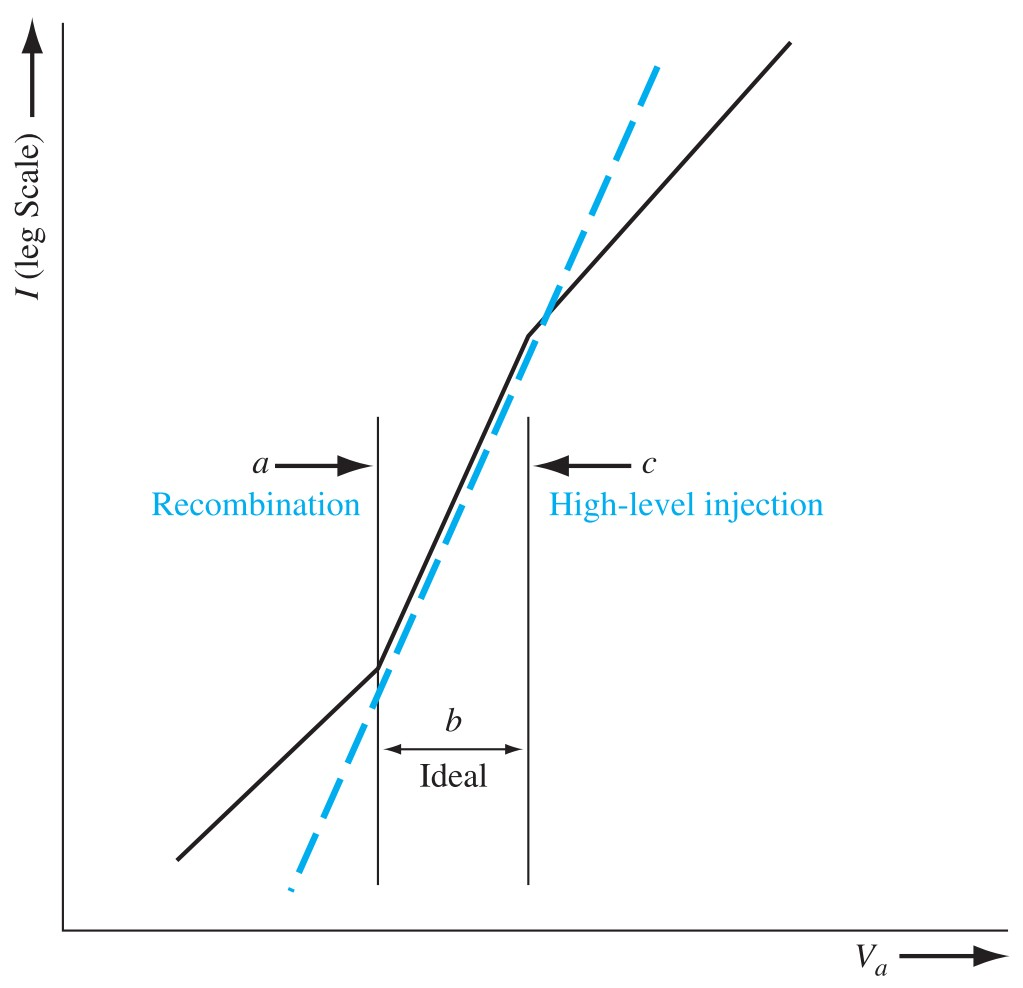
\includegraphics[width=0.6\linewidth]{High-level-injection.jpg} \\
    \end{center}
    %     \centering
    %     \label{fig:High-level-injection.jpg}
    % \end{figure}
    
\section{Chapter 9}
    \begin{minipage}{\linewidth}
        \begin{minipage}{0.45\linewidth}
            \begin{figure}[H]
                \centering
                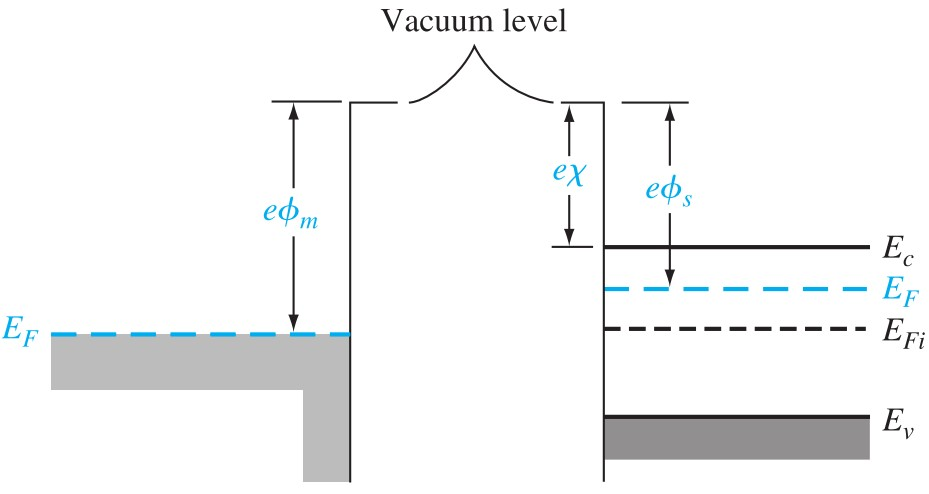
\includegraphics[width=\linewidth]{Work-function-graph.jpg}
                \label{fig:Work-function-graph.jpg}
            \end{figure}
        \end{minipage}
        \begin{minipage}{0.45\linewidth}
            \begin{figure}[H]
                \centering
                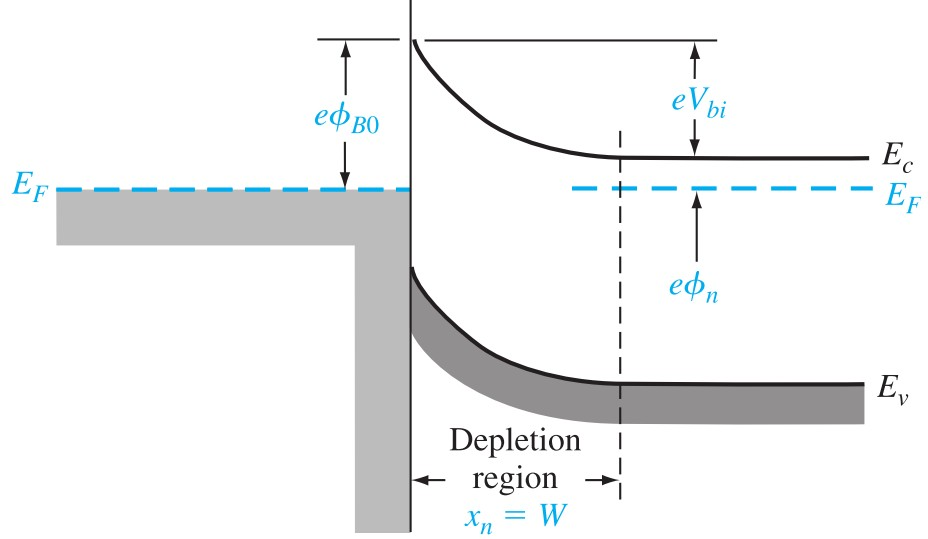
\includegraphics[width=\linewidth]{Ideal-energy-band-diagram-after-contact.jpg}
                \label{fig:Ideal-energy-band-diagram-after-contact.jpg}
            \end{figure}
        \end{minipage}
    \end{minipage}
    Work function: $\phi$ \\
    Electron affinity: $\chi$\\
    Schottky barrier: $\phi_{B0} = \phi_m - \chi$\\
    Built-in potential barrier: $V_{bi} = \phi_{B0} - \phi _n$\\
    $\phi_n = kT \ln \left( \frac{N_c}{N_d} \right)$\\
    
    \par Schottky Barrier Lowering \\
    % \begin{figure}[H]
    %     \centering
        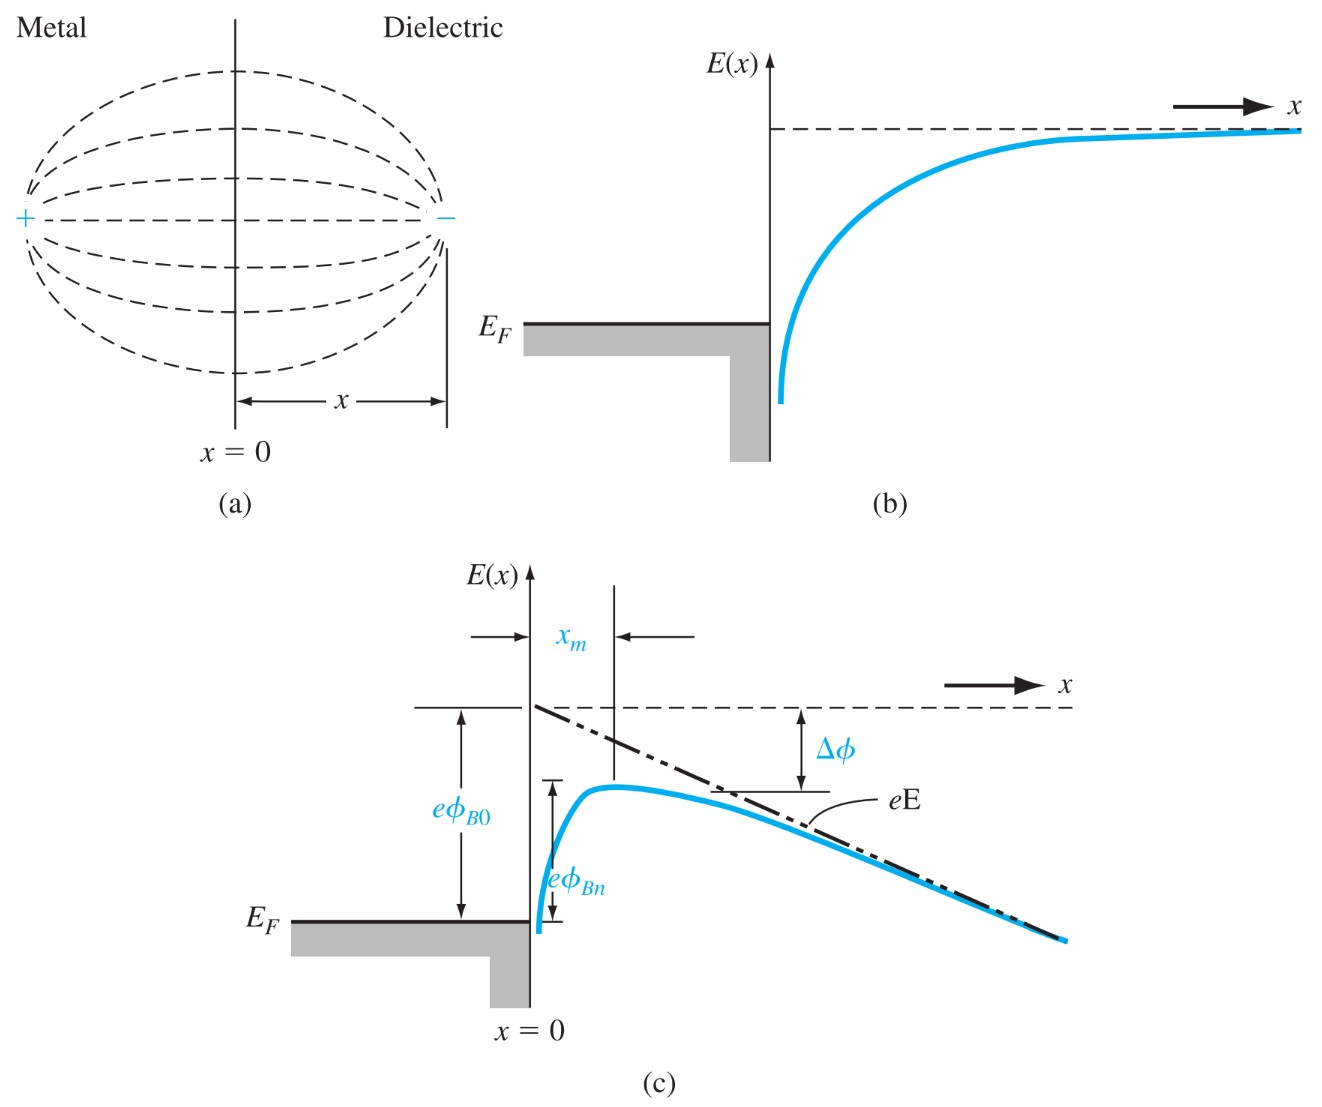
\includegraphics[width=0.9\linewidth]{Schottky-barrier-lowering.jpg}
    %     \label{fig:Schottky-barrier-lowering.jpg}
    % \end{figure}
    \begin{equation*}
        \begin{aligned}
            &F = \frac{-e^2}{4 \pi \varepsilon_s (2x)^2} = -eE \\
            &-\phi(x) = + \int_x^\infty E \d x^\prime = \frac{-e}{16\pi \varepsilon_s x} \\ 
            \text{With electric field: } & -\phi(x) = \frac{-e}{16 \pi \varepsilon_s x} - Ex  \\
            \frac{\d (e \phi(x))}{\d x} = 0 \quad \Rightarrow \quad & \Delta \phi = \sqrt{\frac{eE}{4\pi \varepsilon_s} }  
        \end{aligned}
    \end{equation*}
    
    \par Current-Voltage Relationship 
    \begin{equation*}
        \begin{aligned}
            J &= J_{sT} \left[ \exp\left( \frac{eV_a}{kT}  \right) - 1 \right] \\
            J_{sT} &= A^* T^2 \exp \left( \frac{-e \phi_{Bn} }{kT}  \right) \\
            A^* &= \frac{4\pi e m_n^* k^2}{h^3} 
        \end{aligned}
    \end{equation*}
    $A^*$: effective Richardson constant for thermionic emission. \\
    
    % \begin{figure}[H]
    %     \centering
        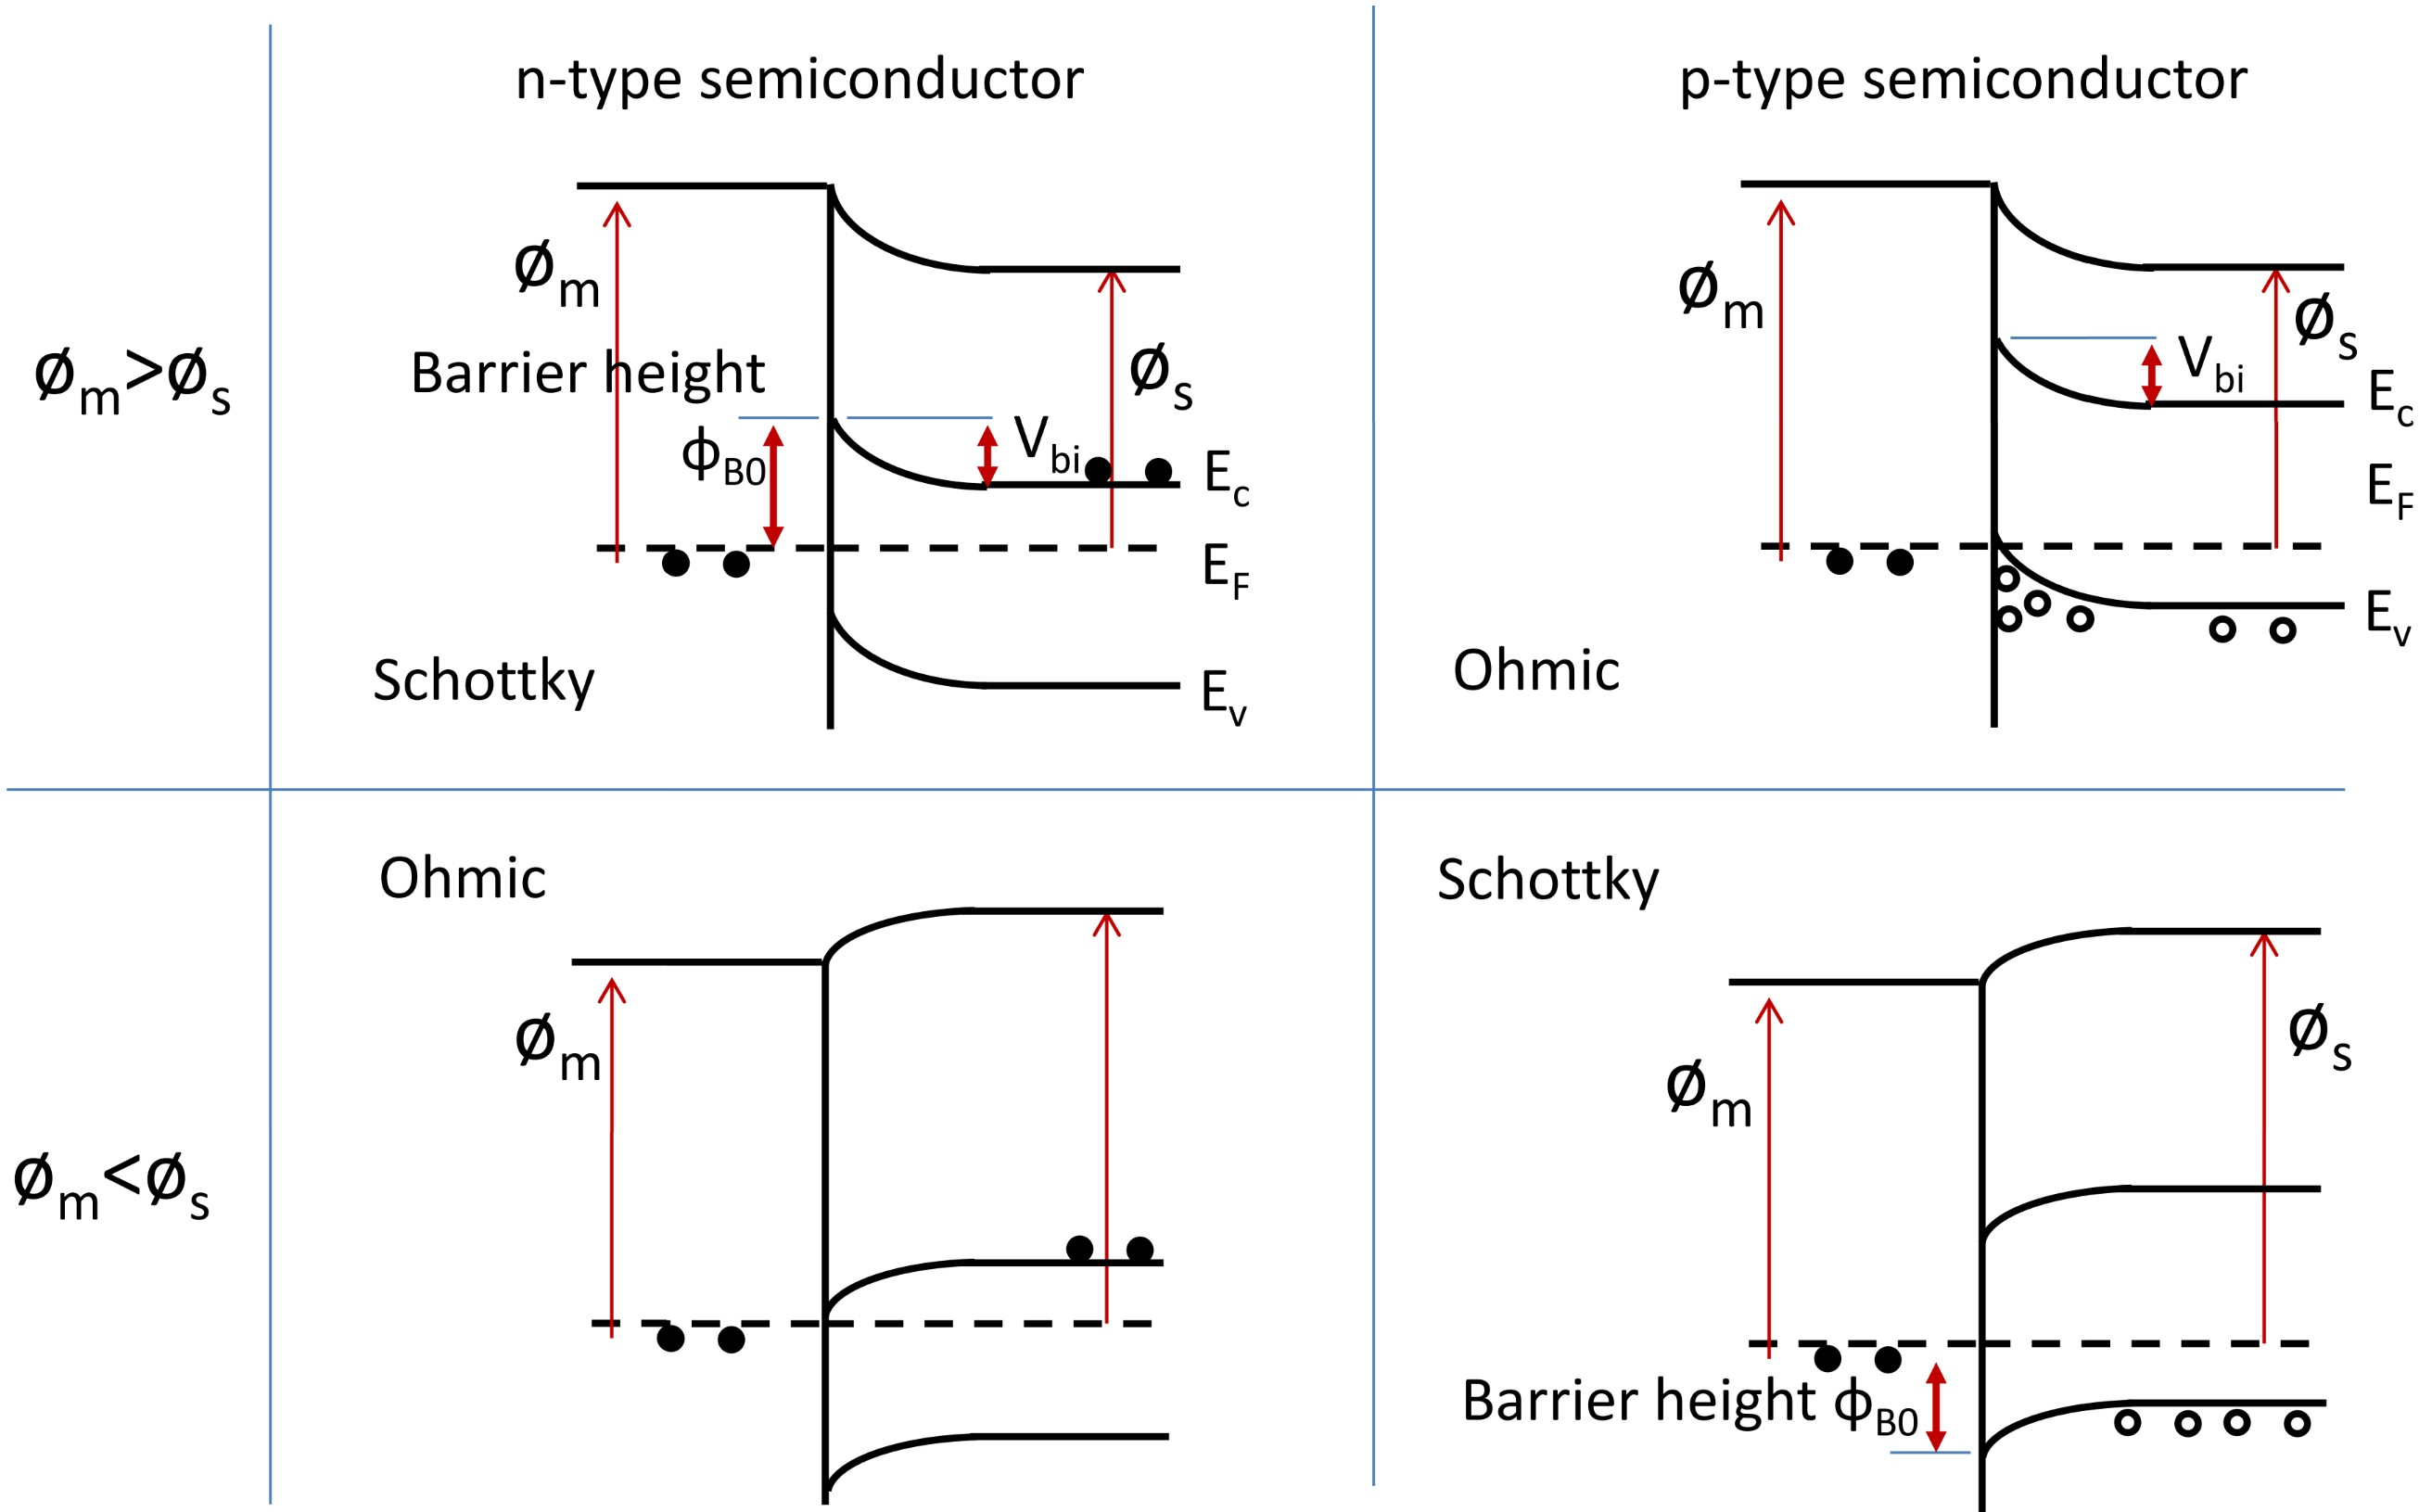
\includegraphics[width=\linewidth]{Types-of-semiconductor.jpg}
    %     \label{fig:Types-of-semiconductor.jpg}
    % \end{figure}
    
    \par Tunneling Barrier \\
    % \begin{figure}[H]
        % \centering
        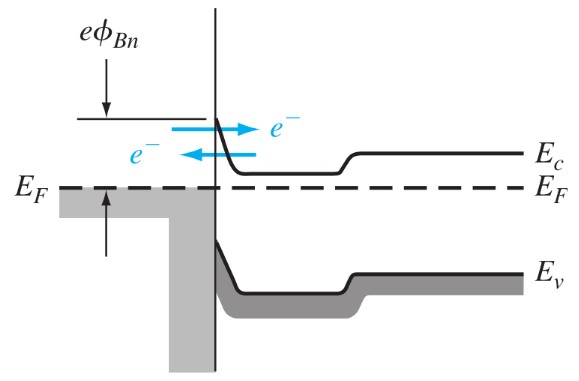
\includegraphics[width=0.8\linewidth]{Tunneling-barrier.jpg}
    %     \label{fig:Tunneling-barrier.jpg}
    % \end{figure}
    \begin{equation*}
        \begin{aligned}
            J_t & \propto \exp \left( \frac{-e \phi_{Bn} }{E_{oo} }  \right) \\
            E_{oo} &= \frac{e \hbar}{2} \sqrt{\frac{N_d}{\varepsilon_s M_n^*} } 
        \end{aligned}
    \end{equation*}
    
    \par Specific Contact Resistance \\
    \begin{equation*}
        \begin{aligned}
            R_c &= \left. \left( \frac{\partial J}{\partial V}  \right)^{-1} \right|_{V = 0} \quad \Omega-cm^{2}  \\
            J_n &= A^* T^2 \exp \left( \frac{-e \phi_{Bn}}{kT}  \right) \left[ \exp \left( \frac{eV}{kT}  \right) - 1 \right] \\
            R_c &= \frac{\left(\frac{kT}{e} \right) \exp \left( \frac{+e \phi_{Bn} }{kT}  \right)}{A^* T^2} 
        \end{aligned}
    \end{equation*}
    $R_c$: the reciprocal of the derivative of current density with respect to voltage evaluated at zero bias.
    \newpage
    \textcolor{white}{a}
    % \newpage
    
    
% 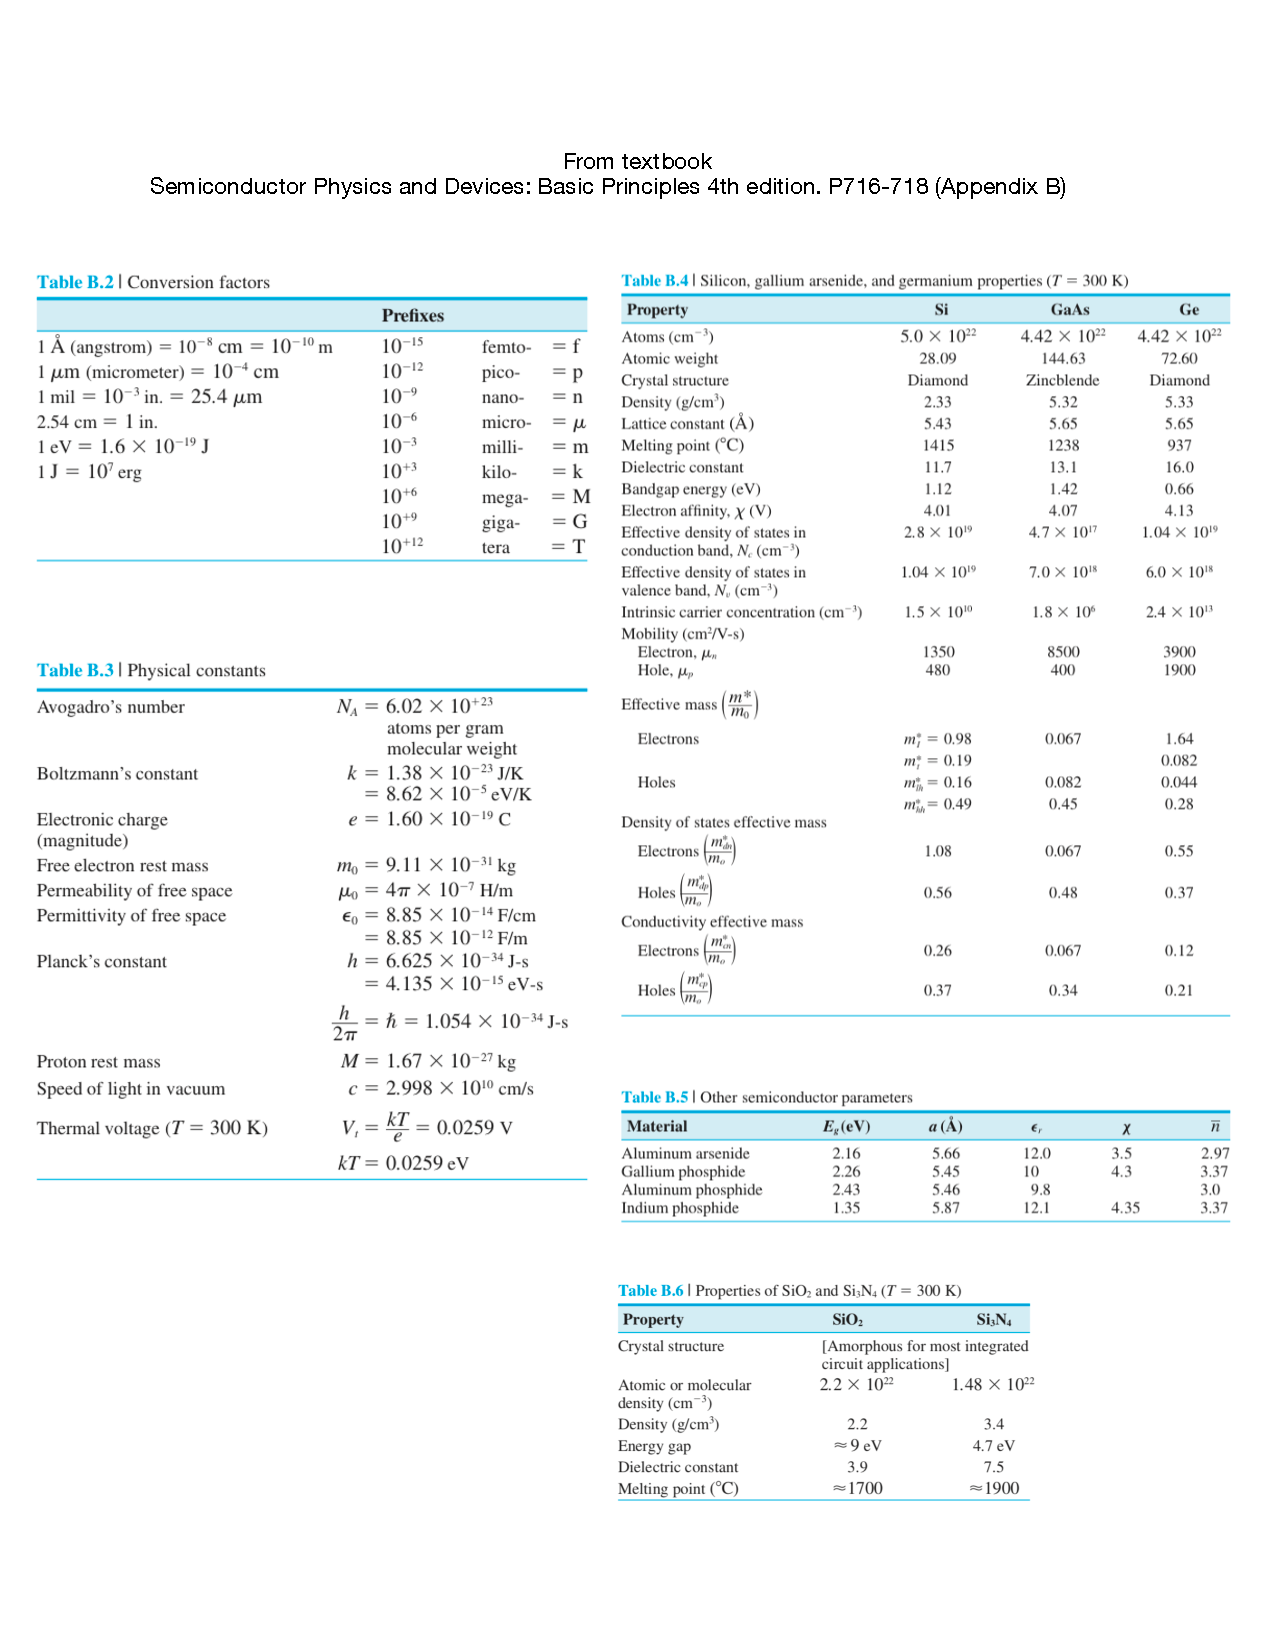
\includepdf[pages = {{}, 1}]{Appendix-mid.pdf}
% 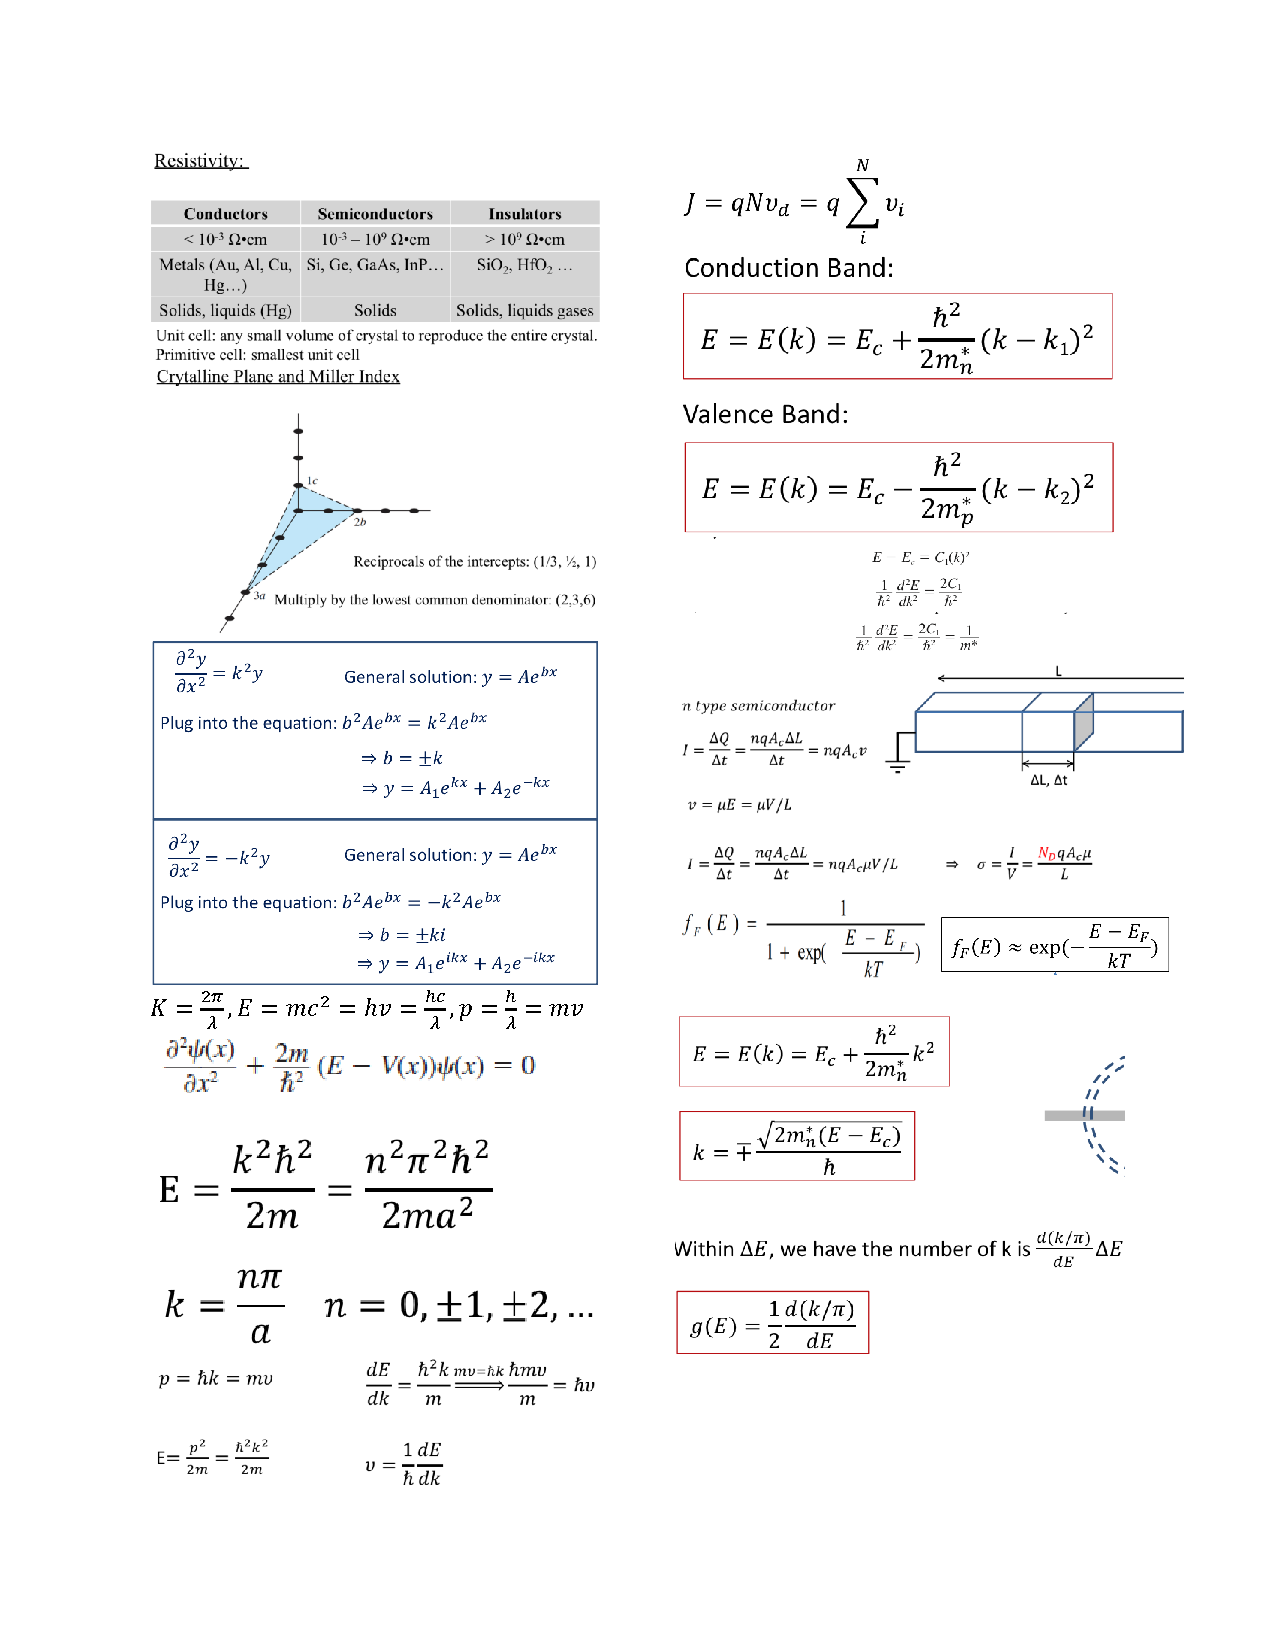
\includepdf[pages=-]{MID1-ctpp_4_06.08.pdf}
% 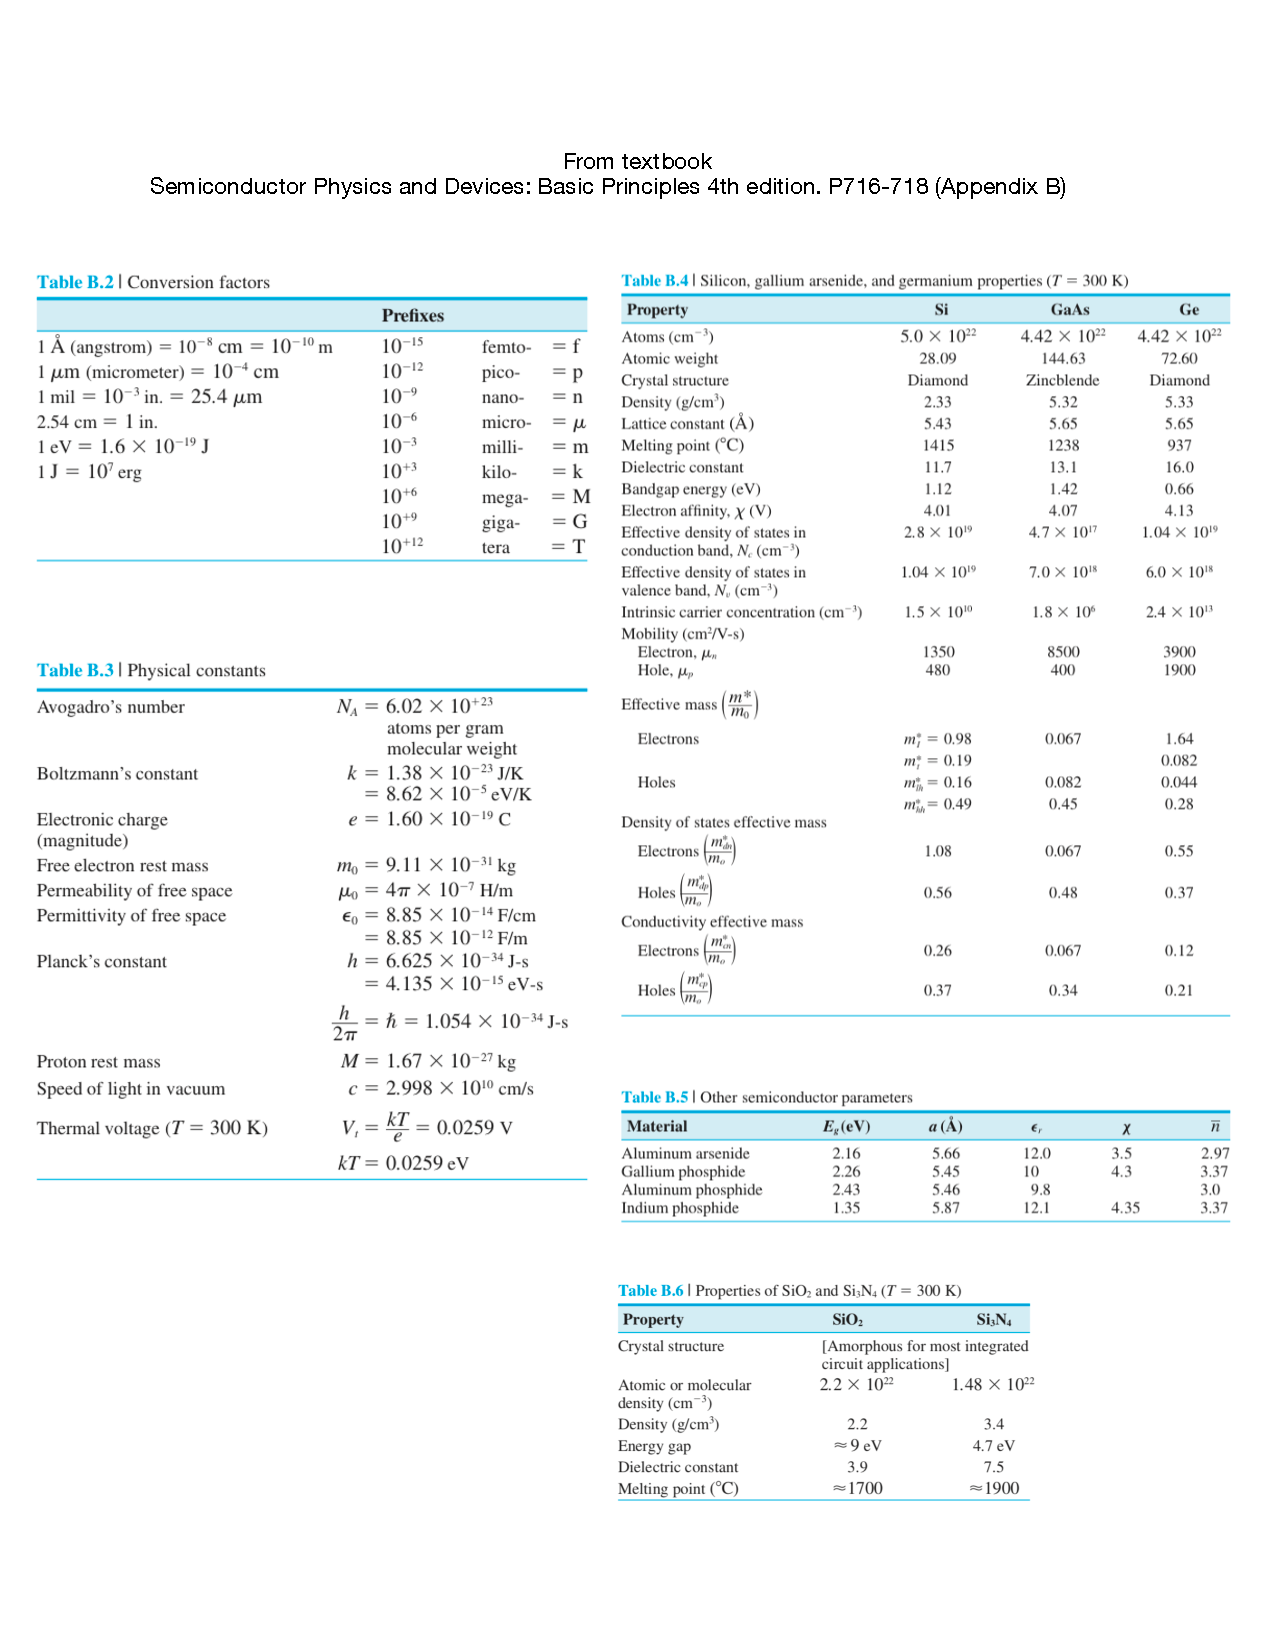
\includepdf[]{Appendix-mid.pdf}
% \newpage
% hello
% 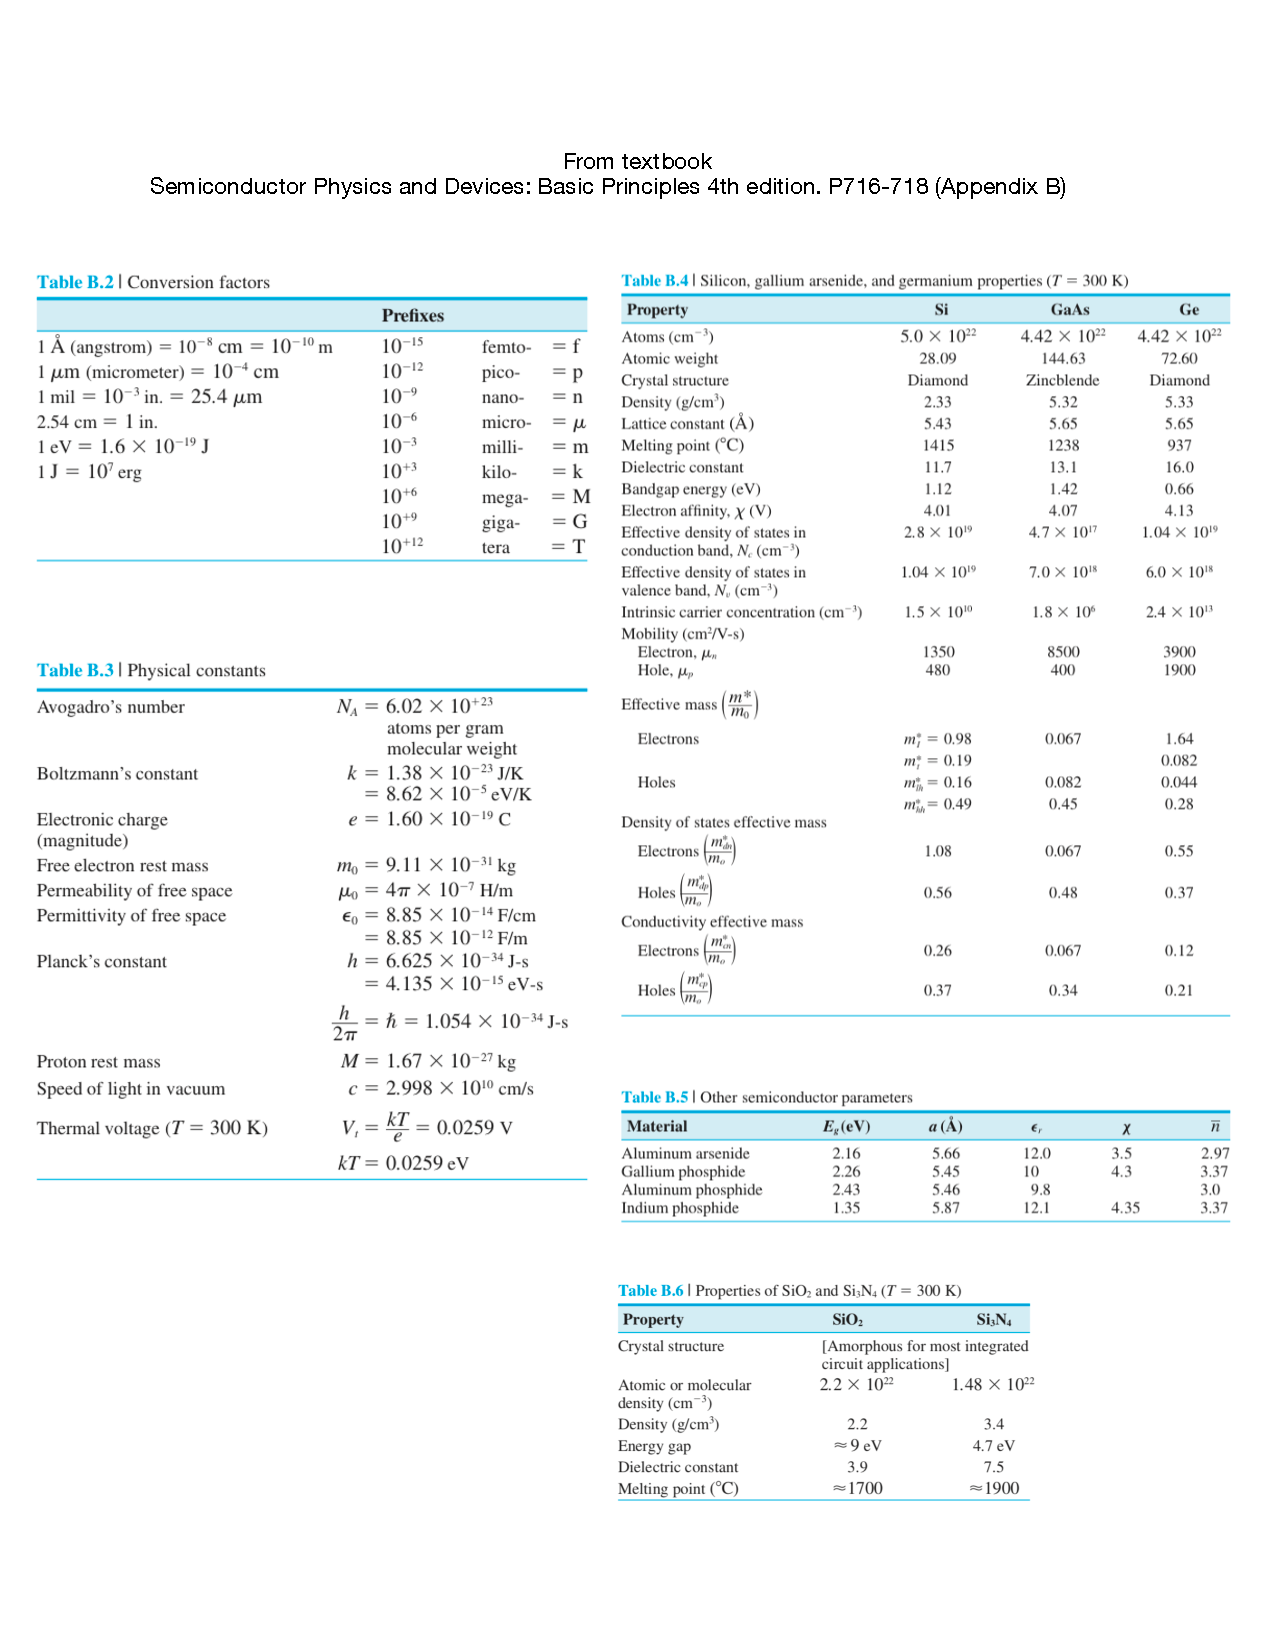
\includegraphics[]{Appendix-mid.pdf}
    
\end{document}